\section{Sesión 9 y Sesión 10}


\subsection{Sucesiones de funciones}
\begin{definicion}
	Una sucesión de funciones $f_n:E\subset \mathbb{R}\to\mathbb{R}$ converge puntualmente en $E_0\subset E$, si $\forall \varepsilon>0\exists N=N(\varepsilon,x)\mathbb{Z}^+\ni$ si $n\geq N\implies |f_n(x)-f(x)|<\varepsilon$. 
	i.e $\lim_{n\to\infty}f_n(x)=f(x)$.
\end{definicion}

\begin{definicion}
	Sea $E\subseteq \mathbb{R}$ y sea la sucesión de funciones $(f_n)$, $f_n:E\to\mathbb{R}$. Se dice que $(f_n)$ converge uniformemente a $f(x),\forall x\in E_0\subset E$, si $\forall \varepsilon >0\exists N=N(\varepsilon)\ni$ si $n\geq N\implies |f_n(x)-f(x)\leq \varepsilon,\forall x\in \varepsilon_0$. Notación $f_n\to_{unif}f$(con dos flechas también).
\end{definicion}

\begin{definicion}(Criterio de Cauchy)
	Sea $E\subseteq \mathbb{R}$ y $(f_n)$ una sucesión de funciones sobre $E$. Entonces, $(f_n)$ converge uniformemente a alguna función $f(x)$ en $E_0\subset E$, ssi $\forall \varepsilon >0\exists N=N(\varepsilon)\in \mathbb{Z}^+\ni $ si $m,n\geq N$, entonces $|f_n(x)-f_m(x)|<\varepsilon,\forall x\in E_0$. 
\end{definicion}

\subsection{Series}

\begin{definicion}
	Se dice que la serie $\sum_{n=1}^\infty a_n$ converge ssi la sucesión de sumas parcial $(s_n)^*$ converge; i.e $\sum a_n$ converge ssi $\lim_{n\to\infty} S_n =L <\infty$. 
	
	
	Dada $\sum_{n=1}^{\infty} a_n, a_n\in \mathbb{R}$, se tiene: 
	\begin{align*}
		S_1 &= a_1\\
		S_2 &= a_1+a_2 = S_1+a_2\\
		S_3 &= a_1 + a_2 + a_3 = S_2+a_3
	\end{align*}
\end{definicion}

\begin{definicion}
	Una serie $\sum_{n=1}^{\infty} a_n$ converge absolutamente, si $\sum_{n=1}^\infty |a_n|$ converge. 
\end{definicion}


\begin{teorema}
	Si la serie $\sum_{n=1}^{\infty}  a_n$ converge absolutamente, entonces la serie converge. 
\end{teorema}

\begin{nota}
	Recuerde el caso de las serie en $\mathbb{C}$. Entonces dada la serie $\sum_{n=1}^{\infty} c_n$, los $c_n\in\mathbb{C}$, se considera la serie $\sum_{n=1}^{\infty}|c_n|$, la cual es una serie de número reales. 
\end{nota}

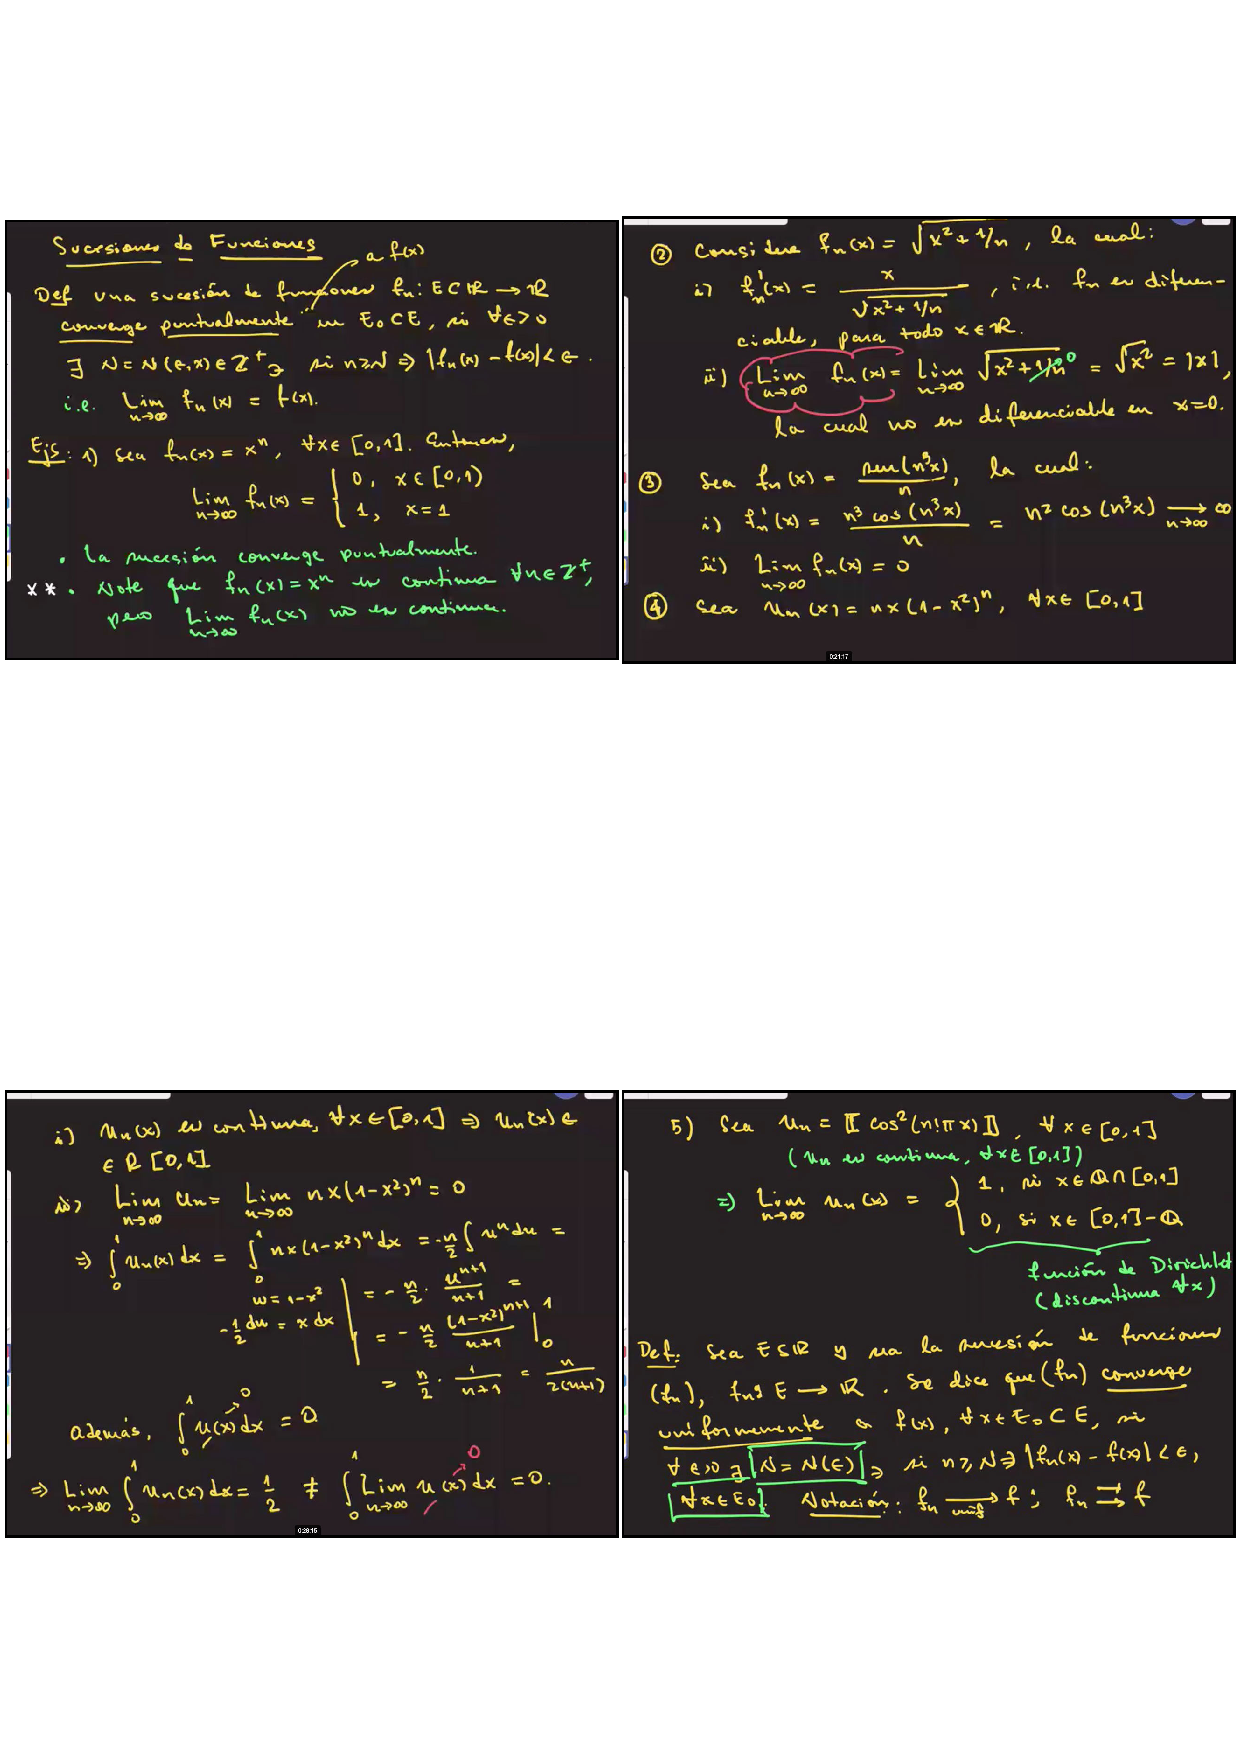
\includepdf[pages=-]{apendices/s9ys10.pdf}